\subsection{Метрические пространства и подпространства}
    \begin{conj}
        $X$ - множество $\rho : X \times X \longrightarrow [0; + \infty)$ - метрика(расстояние)
        если: 
        \begin{enumerate}
            \item $\rho(x, x) = 0 \quad \forall x \in X$
            \item если $\rho(x, y) = 0$, то $x = y$
            \item $\rho(x, y) = \rho(y, x) \quad \forall x, y \in X$
            \item $\rho(x, y) + \rho(y, z) \geqslant \rho(x, z) \quad \forall x, y, z \in X$
        \end{enumerate}
    \end{conj}
\subsubsection*{Примеры}
\begin{enumerate}
    \item Дискретная метрика
        \begin{itemize}
            \item[] $\rho (x, x) = 0$
            \item[] $\rho (x, y) = 1$, если $x \neq y$
        \end{itemize}
    \item $\R \quad \rho (x, y) = \abs{x - y}$
    \item $\R^2 \quad$ обычное расстрояние
    \item Манхэттенская метрика 
    \begin{itemize}
        \item[] $(x', y') = A'$
        \item[] $(x, y) = A$
        \item[] $\rho (A, A') = \abs{x - x'} + \abs{y - y'}$  
    \end{itemize}
    \item Французская железнодорожная метрика \\
    \begin{center}
        \begin{tikzpicture}
            \node (p) {P} node (a) at (-2,1) {A} node (b) at (2,2) {B} node (c) at (1,1) {A}; 
            \draw (p) -- (a); \draw[red,thick] (p) -- (c); \draw[red,thick] (c) -- (b);
        \end{tikzpicture}
        Если $P, A$ и $B$ на луче, то $\rho(AB) = AB$ \\
        \quad \quad \quad Если нет, то $\rho(A, B) = \rho(AP) + \rho(B, P)$
    \end{center}
    \item Расстояние на сфере
\end{enumerate}
\begin{conj}
    Метрическое пространство $(X, \rho), X$ - множество, $\rho$ - метрика на нем
\end{conj}
\begin{conj}
    Подпространство метрического пространства. \\
    $(X, \rho)$ - метрическое пространство, $Y \subset X$ \\
    $(Y, \rho \vert_{Y \times Y})$ - подпространство метрического пространства
    $(X, \rho)$, где $Y$ - подмножество $X$, а $\rho \vert_{Y \times Y}$ - сужение $\rho$ на $Y \times Y$
\end{conj}
\begin{conj} 
    Открытый шар \vspace*{0.5cm} \\
    $B\callout{r}{радиус}(\calloutup{a}{центр шара}) := {x \in X: \rho(x, a) < r}; \quad r > 0$
\end{conj}
\begin{conj} 
    Замкнутый шар \vspace*{0.5cm} \\
    $\overline{B_r}(a) := {x \in X: \rho(x, a) \leqslant r}; \quad r \geqslant 0$ \\
    $B_r(a) \subset \overline{B_r}(a)$
\end{conj}
\begin{itemize}
    \item \underline{Окрестность} точки $a$ - открытый шар $B_r(a)$
\end{itemize}
    \subsubsection*{Примеры} 
    \begin{enumerate}
        \item Дискретная метрика на $X$
        \begin{itemize}
            \item[] $B_{1/2}(a) = {a}$
            \item[] $B_2(a) = X$ 
        \end{itemize}
        \item $\rho(x, y) = |x - y| \quad B_r(a) = (a - r, a + r)$
        \item Манхэттенская метрика
    
        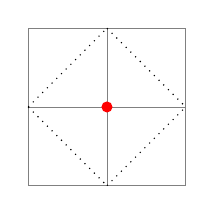
\begin{tikzpicture}
            \draw[help lines] (0,0) grid (2, 2);
            \draw[dotted] (0,1) coordinate (A) -- (1,2) coordinate (B)
            (1,2) -- (2,1);
            \draw[dotted] (0,1) coordinate (A) -- (1,0) coordinate (C)
            (1,0) -- (2,1);
            \fill[red] ((1,1) circle (2pt);
        \end{tikzpicture} \quad $B_r(a)$
    \end{enumerate}
    \subsubsection*{Свойства}
    \begin{enumerate}
        \item $B_r(a) \cap B_R(a) = B_{min\{r, R\}}(a)$
        \item Если $x \neq y$, то найдется $r > 0$, такой, что 
        $\overline{B_r}(x) \cap \overline{B_r}(y) = \varnothing$
        \begin{proof}
            \quad \\
            $r := {{\rho(x, y)}\over{3}}$. Пойдем от противного \\
            Пусть $c \in \overline{B_r}(x) \cap \overline{B_r}(y) \Longrightarrow
            \begin{cases}
                \rho(x, c) \leqslant r \\
                \rho(y, c) \leqslant r
            \end{cases} \Longrightarrow \rho(x, y) \leqslant \rho(x, c) + \rho(y, c) 
            \leqslant 2r = {{2}\over{3}}\rho(x, y)$ - противоречие
        \end{proof}
    \end{enumerate}